\documentclass[10pt]{beamer}

\usetheme[progressbar=frametitle]{metropolis}
\usepackage{appendixnumberbeamer}

\usepackage{booktabs}
\usepackage[scale=2]{ccicons}

\usepackage{pgfplots}
\usepgfplotslibrary{dateplot}

% \usepackage{natbib}

\usepackage{xspace}
\newcommand{\themename}{\textbf{\textsc{metropolis}}\xspace}

\title{Taxing the upzone:}
\subtitle{Cash proffers and housing supply}
\date{\today}
% \date{}
\author{Colin Williams}
\institute{University of Virginia}
% \titlegraphic{\hfill\includegraphics[height=1.5cm]{logo.pdf}}

\begin{document}

\maketitle

\begin{frame}{Zoning and The Coase Theorem}
    For locals, many negative externalities from residential land use:
    \begin{itemize}
        \item High marginal infrastructure costs (schools, roads, etc.)
        \item Noise, shade, parking, traffic congestion
        \item ``Business-stealing'' -- new supply lowers price of existing housing stock
    \end{itemize}
    \vspace{2em}
    Local government has zoning authority $\implies$ property rights are well defined

    \vspace{2em}
    Why don't we see more welfare-enhancing trades?
\end{frame}


\begin{frame}
    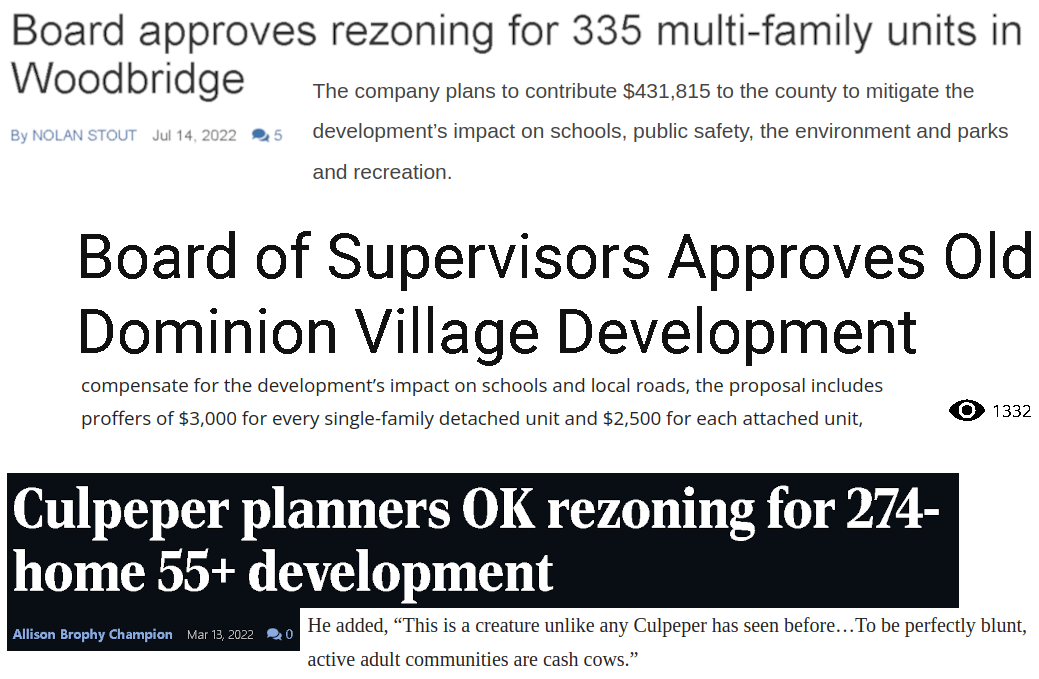
\includegraphics[width=\textwidth]{figures/images/20230312 Rezoning News VA.png}
\end{frame}

\begin{frame}{VA Proffer Reform Act of 2016}

``Impact fees'' broadly illegal in VA $\implies$ localities rely on ``voluntary'' proffers tied to a rezoning application
\vspace{2em}

In 2016, builders were uphappy with large cash proffers, lobbied state legislature for reform:
\begin{itemize}
    \item Proffers must address an impact that is \textit{specifically attributable} to the proposed development
    \item Applies to all residential rezoning applications filed after July 1, 2016 (small parts of NOVA are excepted)
\end{itemize}
\end{frame}

\begin{frame}{Reform has chilling effect on proffer revenues}
    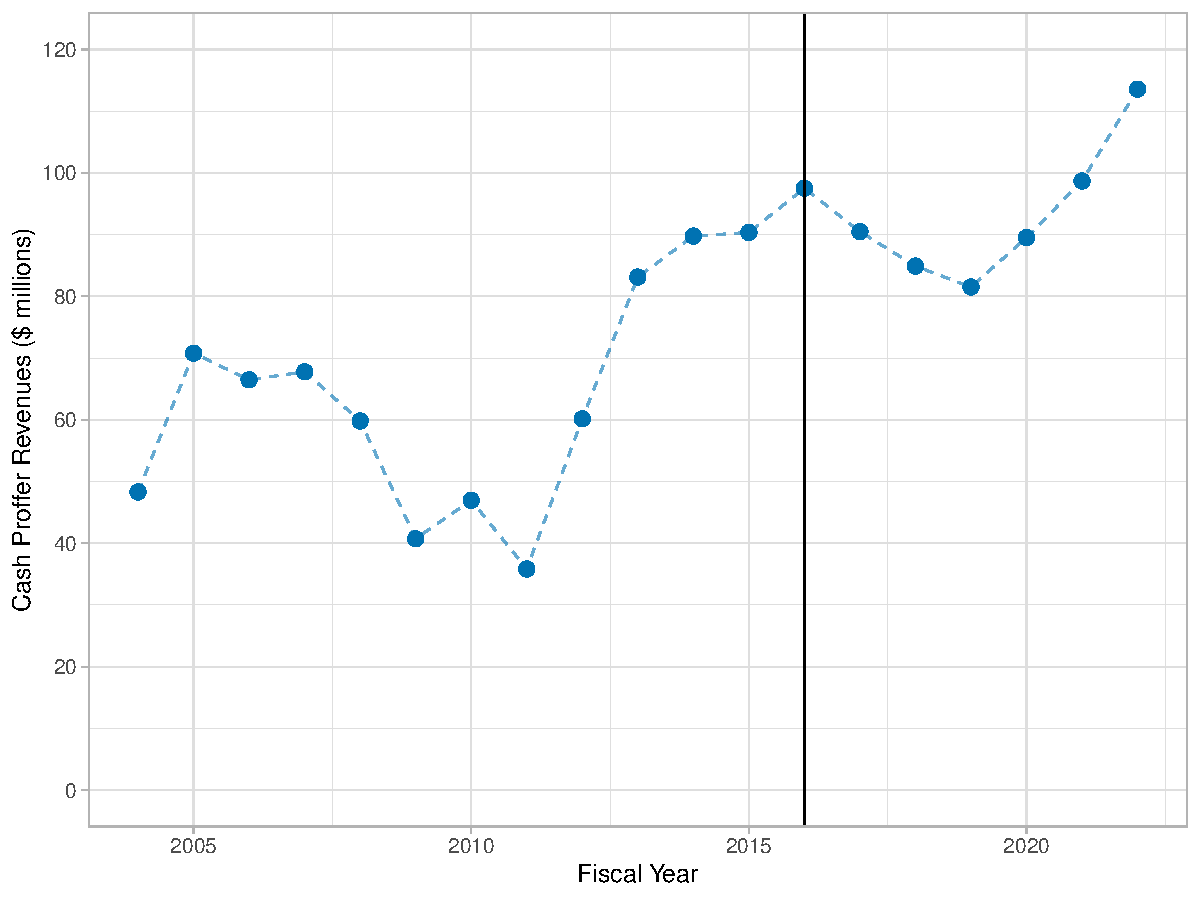
\includegraphics[width=\textwidth]{figures/proffer_revenues.pdf}
\end{frame}

\begin{frame}[t]{What happens to housing construction?}
    Estimate an event study specification: $$log(Permits_{jt} + 1) = \sum_{t=2011q3}^{2019q2}\beta_t(Proffers16_j \times I_t) + \gamma_j + \delta_t + \epsilon_{jt}$$

    where for county $j$ in year-quarter $t$:
    \begin{itemize}
        \item $Permits_{jt}$ is the number of approved single-family building permits
        \item $Proffers16_j$ indicates VA counties in which pre-reform proffer revenue exceeded 1\% of assessed value of all approved housing units 
        \item $I_t$ is a set of year-quarter indicators
        \item $\gamma_j$, $\delta_t$ are county and time fixed-effects
    \end{itemize}
    
\end{frame}

\begin{frame}{Single family permits fall with a lag}
    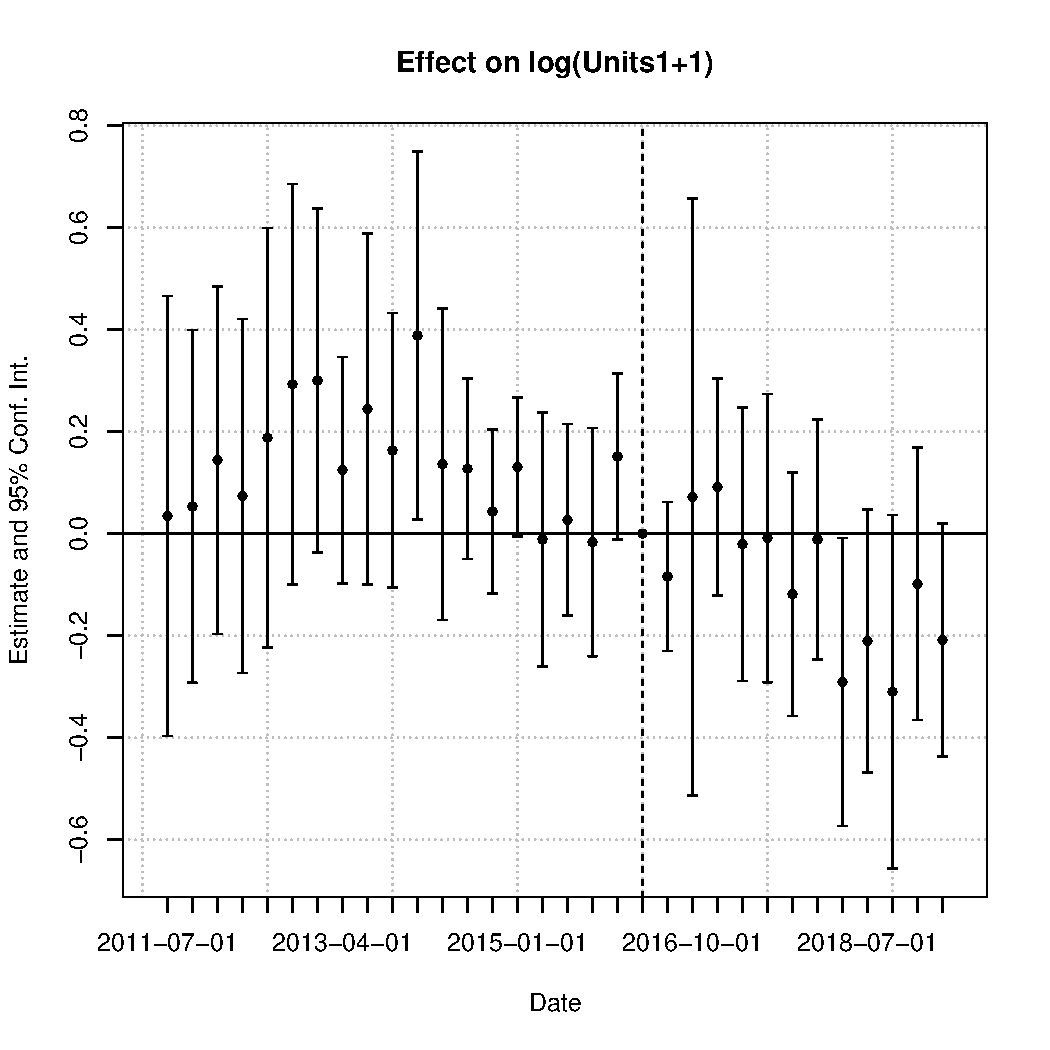
\includegraphics[width=\textwidth, height = \textheight]{figures/eventstudy_units1.pdf}
\end{frame}

\begin{frame}{Synthetic DiD (Arkhangelsky et al 2021)}
    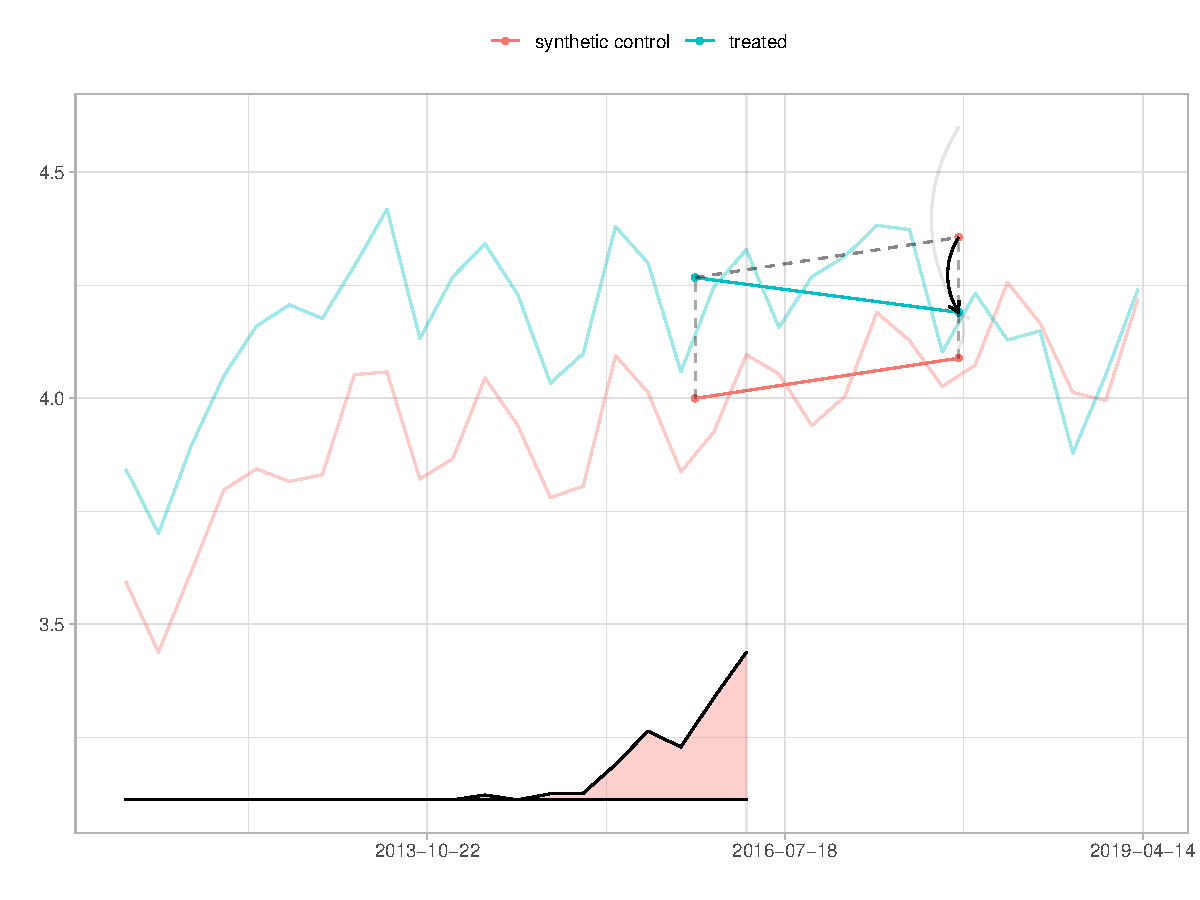
\includegraphics[width=\textwidth, height = \textheight]{figures/synthdid.pdf}
\end{frame}

\begin{frame}{Discussion}
Synthetic DiD looks OK, but effect is imprecise: 
\begin{itemize}
    \item Census Building Permit Survey data are noisy
    \item Developers anticipated reform, rushed to file applications before law takes effect
    \item Rezoning negotiations are protracted $\implies$ small immediate impact
\end{itemize}
\vspace{2em}
Solution: collect data on rezoning applications and ordinances to clarify mechanism
\end{frame}

\begin{frame}{Data on Rezoning Activity}
    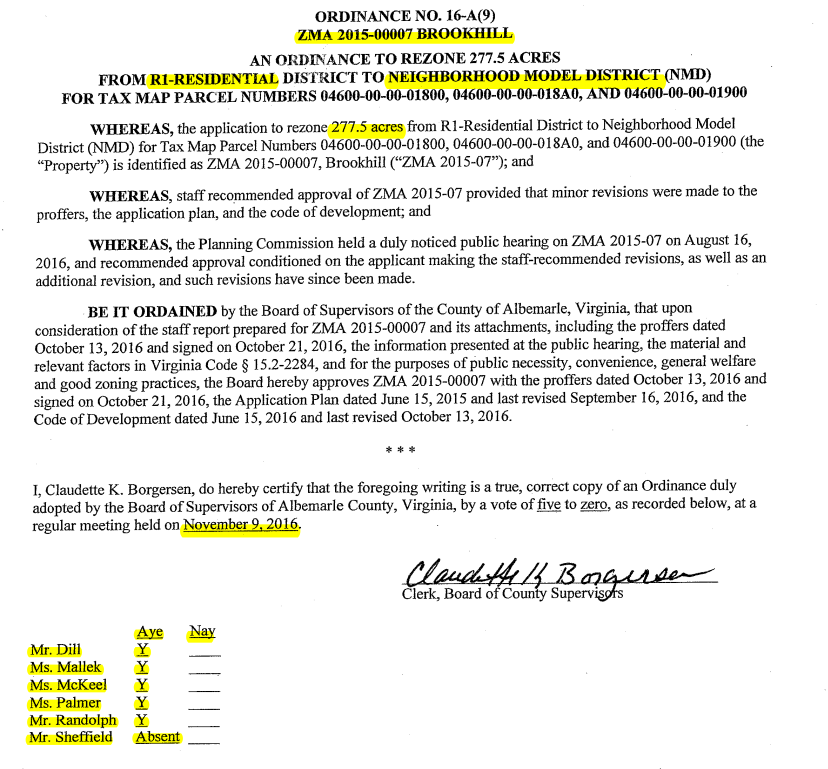
\includegraphics[width=\textwidth]{figures/images/rezoning_example1.png}
\end{frame}

\begin{frame}{Data on Rezoning Activity}
    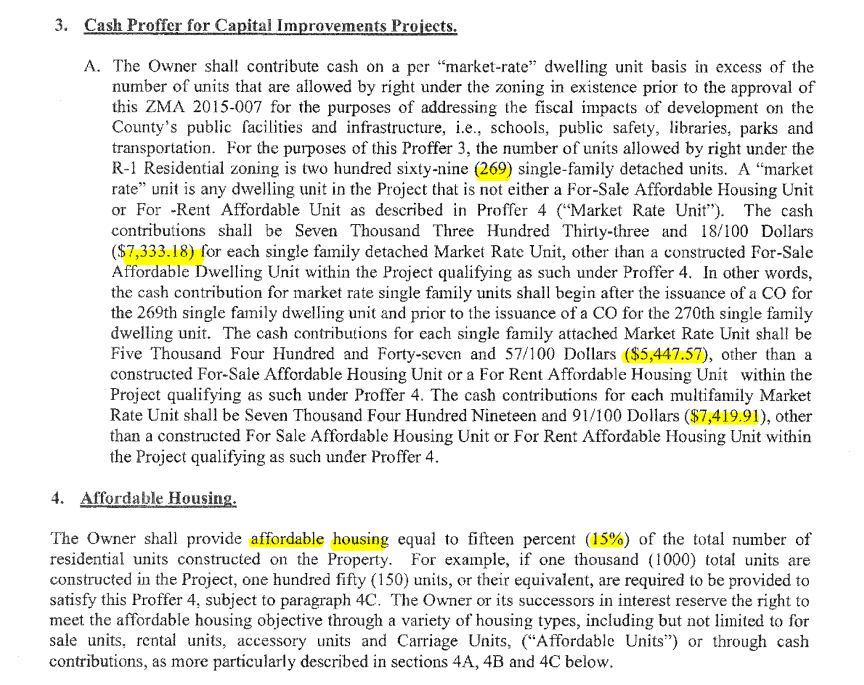
\includegraphics[width=\textwidth]{figures/images/rezoning_example2.png}
\end{frame}

\begin{frame}{Chesterfield County}
    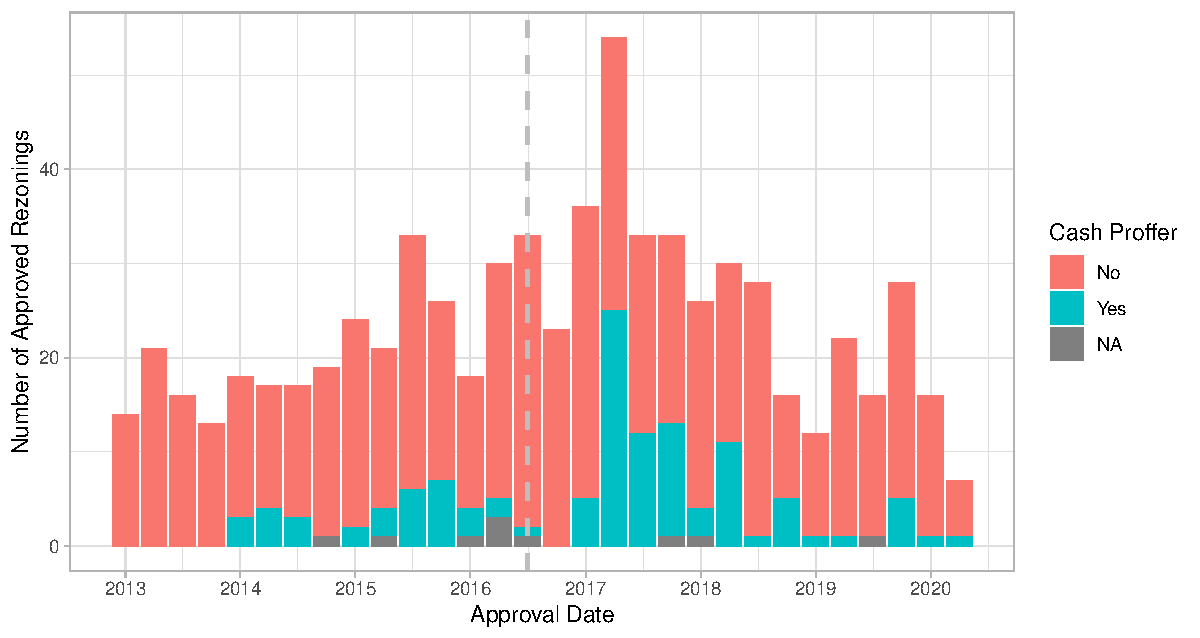
\includegraphics[width=\textwidth]{figures/plot_chesterfield_approvals.pdf}
\end{frame}

\begin{frame}{Fairfax County}
    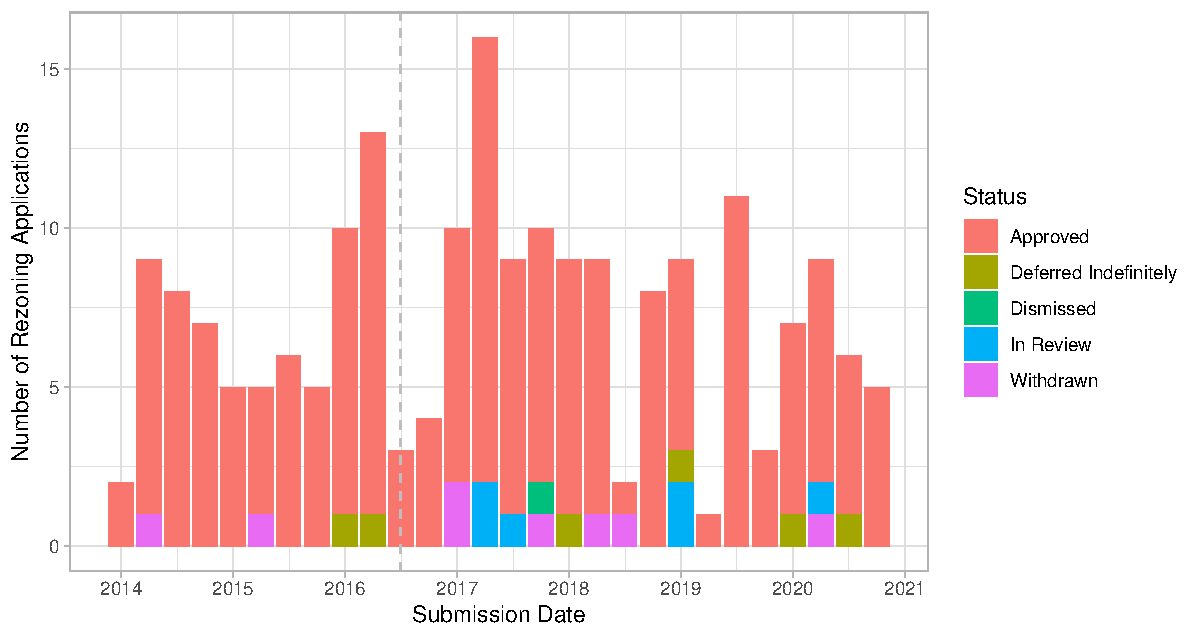
\includegraphics[width=\textwidth]{figures/plot_fairfaxco_submissions.pdf}
\end{frame}

\begin{frame}{Why Bother?}
\textbf{Concern:} Given weak evidence on housing permits (i.e., the outcome we actually care about), why bother collecting data on rezoning activity?
\vspace{2em}

A null result could be informative: rezoning not actually a bottleneck in housing supply? Or was reform just a minor blip?

\vspace{2em}
VA proffer regime is unusual, but impact fees widespread across US (although perhaps the only zoning regulation that is declining in popularity)

\vspace{2em}
``Discrete-choice'' type data offer a chance to denominate locality preferences over land uses in dollar terms.

\end{frame}


\end{document}


